\chapter{Proposed Methodology}
The proposed project will follow a structured, sequential methodology to transform raw medical text into accurate specialty predictions.

\section{Dataset}
The system will utilize the Medical Transcriptions (MTSamples) dataset. This publicly available corpus contains around 5,000 medical transcription reports spanning various clinical specialties. It appropriately exemplifies the complexities and imbalances inherent in real-world clinical documentation. The dataset consists of unstructured clinical narratives dictated by healthcare professionals, covering diverse medical domains such as Surgery, Cardiology, and Neurology. Because it accurately mirrors the linguistic structure of actual patient records, it is highly suitable for evaluating traditional NLP and machine learning approaches.

\section{Data Preprocessing}
Recognizing that raw clinical text cannot be directly ingested by mathematical models, a rigorous preprocessing pipeline will be executed:
\begin{itemize}
    \item \textbf{Lowercasing:} Converting all text to lowercase to ensure uniform mathematical treatment of words regardless of capitalization.
    \item \textbf{Tokenization:} Fracturing continuous clinical narratives into discrete word units (tokens) using NLP libraries.
    \item \textbf{Stop-word removal:} Systematically filtering out common, non-informative English vocabulary that dilutes the predictive power of the dataset.
    \item \textbf{Lemmatization:} Reducing all remaining clinical tokens to their absolute linguistic root forms (e.g., converting ``operating'' and ``operated'' to ``operate'').
\end{itemize}

\section{TF-IDF Feature Extraction}
Following preprocessing, the system will systematically apply Term Frequency-Inverse Document Frequency (TF-IDF) vectorization. This statistical technique will evaluate the entire clinical corpus to generate high-dimensional numerical feature vectors. TF-IDF explicitly highlights unique, highly discriminative medical terminology specific to particular specialties while mathematically suppressing ubiquitous words, appropriately structuring the data for algorithmic ingestion.

\section{Machine Learning Models}
The core computational engine will independently train four traditional machine learning classifiers on the extracted TF-IDF feature space:
\begin{itemize}
    \item \textbf{Logistic Regression:} A robust linear model highly effective for high-dimensional text classification.
    \item \textbf{Support Vector Machine (SVM):} An algorithm that attempts to find the optimal mathematical hyperplane to separate different medical specialty classes.
    \item \textbf{Random Forest:} A tree-based ensemble method that reduces overfitting by averaging multiple decision trees.
    \item \textbf{Multinomial Naïve Bayes:} A probabilistic classifier particularly suited for word frequency features.
\end{itemize}

\section{Voting Ensemble Classifier}
Building upon the independently trained baselines, a Hard Voting Ensemble Classifier will be developed. This architecture will effectively combine the multiple classifiers into a unified predictive system. By aggregating the discrete class predictions of the individual models and calculating the absolute statistical majority, the ensemble framework will mathematically mitigate individual algorithmic biases, yielding a significantly more stable and accurate final prediction.

\section{Flask Web Application}
To ensure practical accessibility, a responsive web interface will be constructed utilizing HTML, CSS, and the lightweight Python Flask framework. The serialized ensemble model and TF-IDF vectorizers will be integrated into the backend, allowing users to efficiently input raw medical text and instantly receive the predicted medical specialty.

\section{Evaluation Strategy}
The system will be subjected to rigorous statistical evaluation using an unseen testing dataset. Performance will be quantified using standard classification metrics:
\begin{itemize}
    \item \textbf{Accuracy:} The overall percentage of correctly classified reports.
    \item \textbf{Precision:} The proportion of true positive predictions among all positive predictions for a given specialty.
    \item \textbf{Recall:} The proportion of true positive predictions among all actual instances of a given specialty.
    \item \textbf{F1-score:} The harmonic mean of Precision and Recall, crucial for evaluating performance on the imbalanced MTSamples dataset.
\end{itemize}

\section{Proposed Workflow}

\begin{figure}[htbp]
\centering
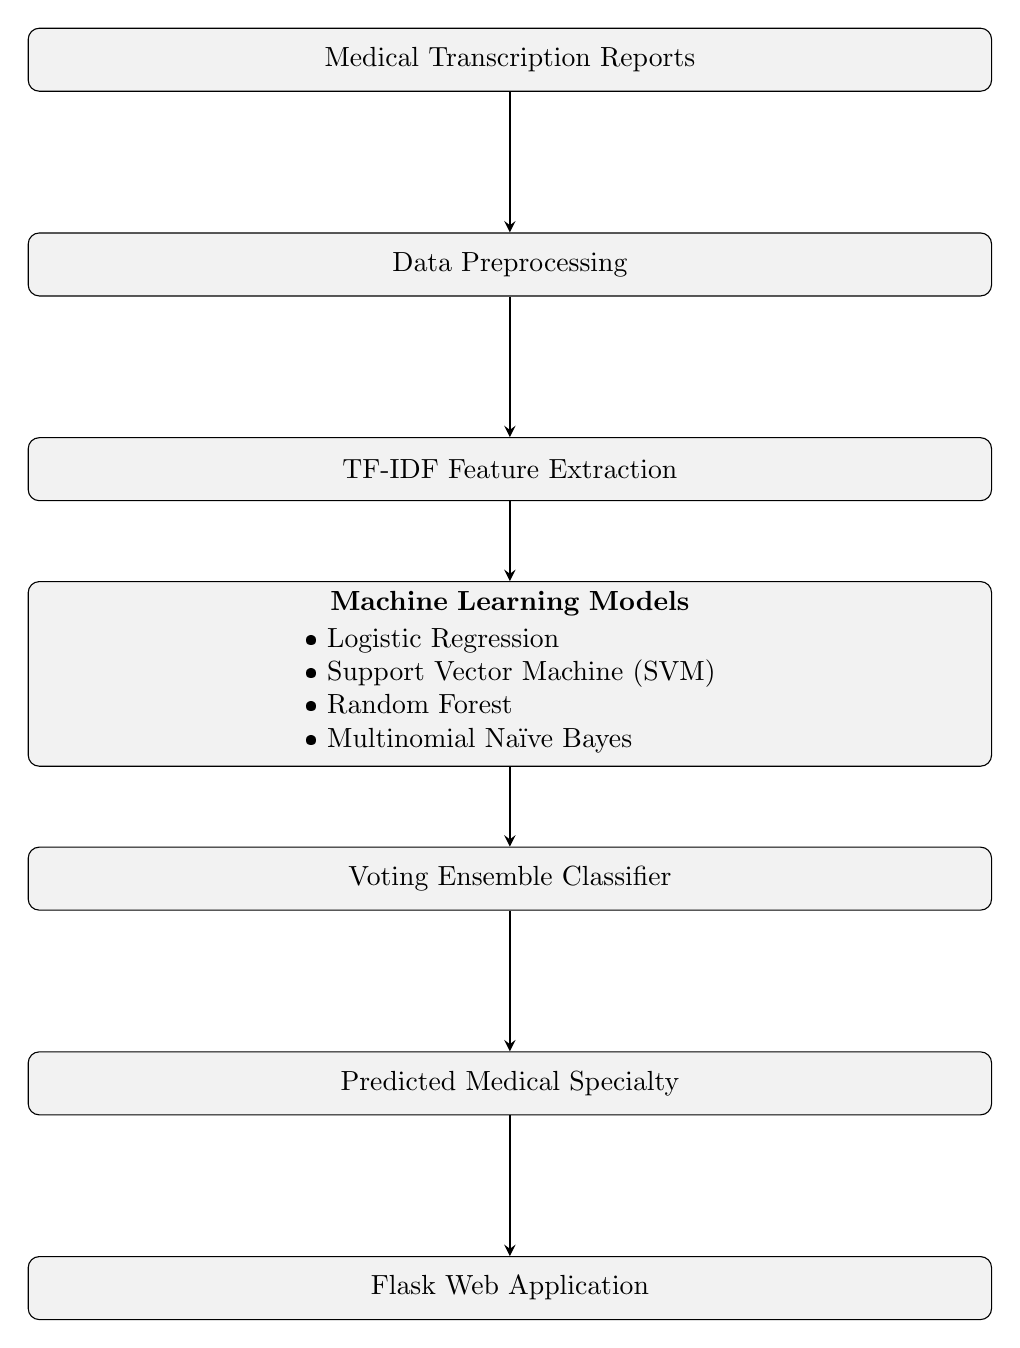
\begin{tikzpicture}[
    node distance=2.6cm,
    box/.style={rectangle, draw, rounded corners, text width=12cm, align=center, minimum height=0.8cm, fill=gray!10},
    arrow/.style={thick,->,>=stealth}
]

\node (data) [box] {Medical Transcription Reports};
\node (prep) [box, below of=data] {Data Preprocessing};
\node (tfidf) [box, below of=prep] {TF-IDF Feature Extraction};
\node (models) [box, below of=tfidf] {\textbf{Machine Learning Models} \\[0.5ex] \begin{tabular}{l} \textbullet~Logistic Regression \\ \textbullet~Support Vector Machine (SVM) \\ \textbullet~Random Forest \\ \textbullet~Multinomial Naïve Bayes \end{tabular}};
\node (ensemble) [box, below of=models] {Voting Ensemble Classifier};
\node (output) [box, below of=ensemble] {Predicted Medical Specialty};
\node (flask) [box, below of=output] {Flask Web Application};

\draw [arrow] (data) -- (prep);
\draw [arrow] (prep) -- (tfidf);
\draw [arrow] (tfidf) -- (models);
\draw [arrow] (models) -- (ensemble);
\draw [arrow] (ensemble) -- (output);
\draw [arrow] (output) -- (flask);

\end{tikzpicture}
\caption{Overall Workflow of the Proposed System}
\end{figure}

The complete system workflow follows a linear pipeline: Medical transcription data is ingested and rigorously cleaned through the NLP preprocessing stage. The standardized text is mathematically vectorized via TF-IDF into high-dimensional numerical features. These features are simultaneously evaluated by Logistic Regression, SVM, Random Forest, and Naïve Bayes algorithms. Their independent predictions are aggregated by the Voting Ensemble Classifier to produce the final, definitive medical specialty classification. This entire prediction engine is ultimately served via the Flask web interface for end-user interaction.
